\section[Рисунки]{Растровая графика}
\subsection[Математика]{История математики, это 1 картинка}

\ifpdf
	\begin{center} 
		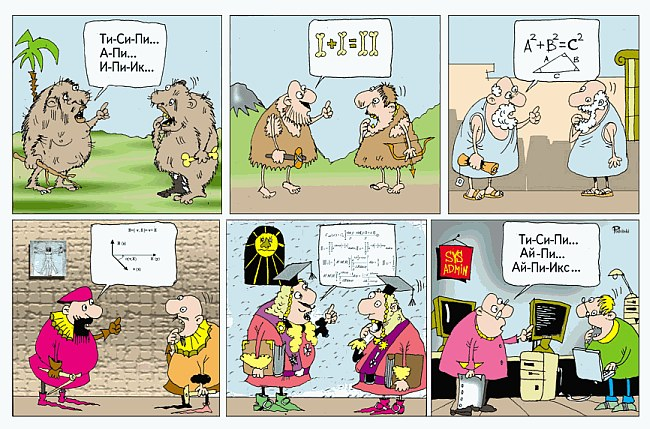
\includegraphics[width=15cm]{img/math.jpg}
	\end{center}
	
%\lstinputlisting[language=Tex]{src/part02.tex}		

\begin{lstlisting}
\subsection[Математика]{История математики, это 1 картинка}
	\begin{center} 
		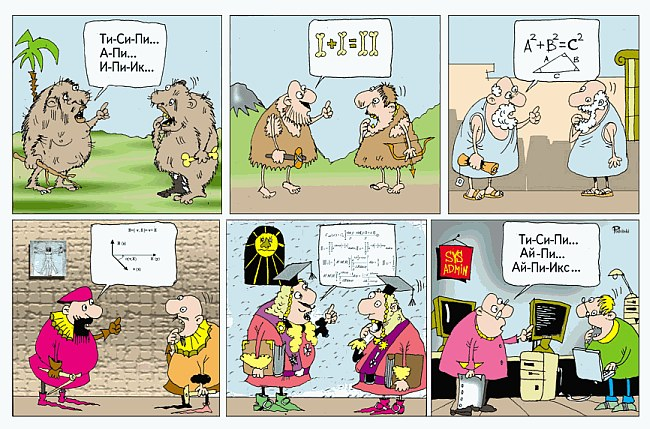
\includegraphics[width=15cm]{img/math}
	\end{center}
\subsection{Пророчество}
	\begin{center} 
		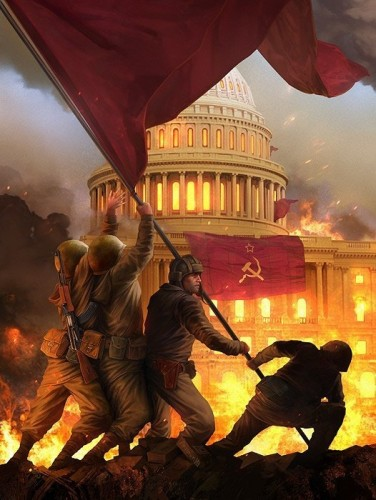
\includegraphics[height=100mm]{img/theFutureofUsa}
	\end{center}
\subsection[Оси]{Оси и отрезки}
	\begin{center} 
		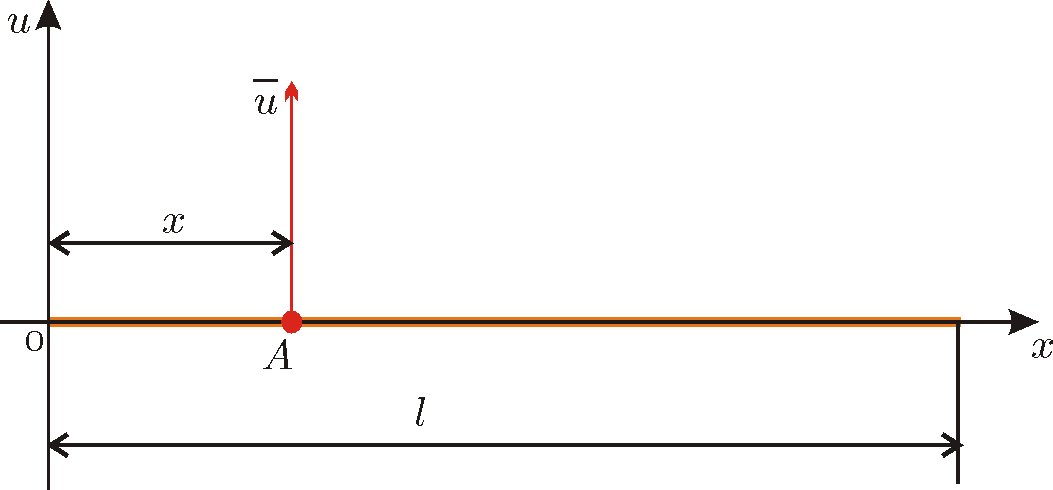
\includegraphics[width=6.3in]{img/l2-1-1}
	\end{center}
\pagebreak %% Разрыв страницы :-)

\end{lstlisting}

\subsection{Пророчество}
	\begin{center} 
		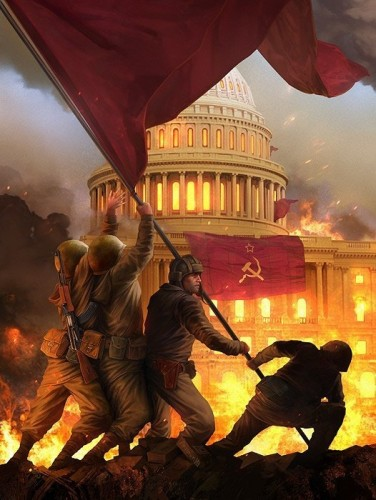
\includegraphics[height=100mm]{img/theFutureofUsa.jpg}
	\end{center}
\subsection[Оси]{Оси и отрезки}
	\begin{center} 
		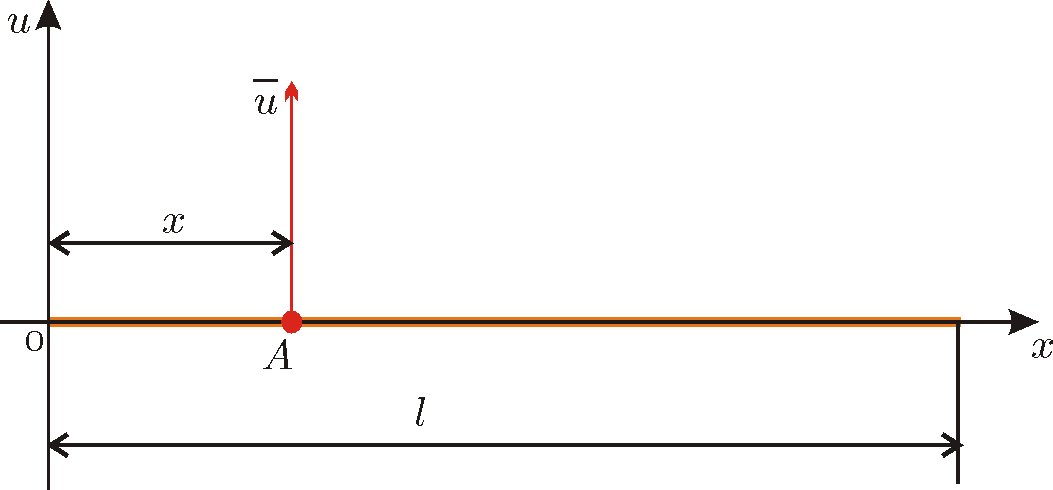
\includegraphics[width=6.3in]{img/l2-1-1.png}
	\end{center}
	
\else
	Нет картинок. \LaTeX \ не дружит с \textit{png}, \textit{jpg} и пр.
	Конвертируйте в \textit{*.*ps*.}
\fi

\pagebreak %% Разрыв страницы :-)
